% arara: latex: { interaction: nonstopmode, options: ['-halt-on-error'] }
% arara: dvisvgm: { options: ['--no-fonts', '--bbox=papersize', '--zoom=-1'] }
% Vector reconstruction of the original 400 x 400 PNG.
% Coordinates are scaled by 1/100, with the vertical axis reversed.
% From this directory: latex triangulation-1.tex
% dvisvgm --no-fonts --bbox=papersize --zoom=-1 triangulation-1.dvi
\documentclass[tikz,border=0pt]{standalone}
\tikzset{
  empty circle/.style={draw=black!40,line width=0.55pt},
  edge/.style={draw=black,line width=1.05pt,line cap=round,line join=round},
}

\newcommand{\site}[3]{%
  \expandafter\def\csname site#1x\endcsname{#2}%
  \expandafter\def\csname site#1y\endcsname{#3}%
  \coordinate (#1) at (#2,#3);
}

% Compute each circumcircle from its three sites so the source stays editable.
\newcommand{\circumcircle}[3]{%
  \pgfmathsetmacro{\ax}{\csname site#1x\endcsname}
  \pgfmathsetmacro{\ay}{\csname site#1y\endcsname}
  \pgfmathsetmacro{\bx}{\csname site#2x\endcsname}
  \pgfmathsetmacro{\by}{\csname site#2y\endcsname}
  \pgfmathsetmacro{\cx}{\csname site#3x\endcsname}
  \pgfmathsetmacro{\cy}{\csname site#3y\endcsname}
  \pgfmathsetmacro{\aa}{\ax*\ax+\ay*\ay}
  \pgfmathsetmacro{\bb}{\bx*\bx+\by*\by}
  \pgfmathsetmacro{\cc}{\cx*\cx+\cy*\cy}
  \pgfmathsetmacro{\dd}{2*(\ax*(\by-\cy)+\bx*(\cy-\ay)+\cx*(\ay-\by))}
  \pgfmathsetmacro{\ux}{(\aa*(\by-\cy)+\bb*(\cy-\ay)+\cc*(\ay-\by))/\dd}
  \pgfmathsetmacro{\uy}{(\aa*(\cx-\bx)+\bb*(\ax-\cx)+\cc*(\bx-\ax))/\dd}
  \pgfmathsetmacro{\rr}{sqrt((\ux-\ax)^2+(\uy-\ay)^2)}
  \draw[empty circle] (\ux,\uy) circle[radius={\rr*2.5cm}];
}

\begin{document}
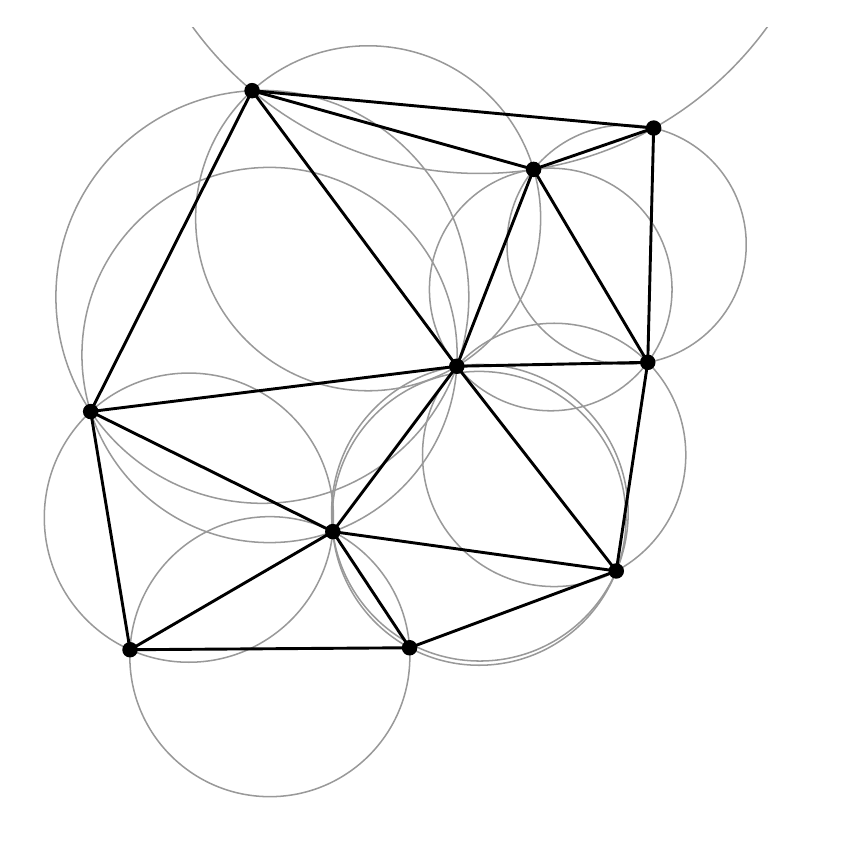
\begin{tikzpicture}[x=2.5cm,y=2.5cm]
  % Keep the original square crop and transparent background.
  \path[use as bounding box] (0,0) rectangle (4,-4);
  \clip (0,0) rectangle (4,-4);

  \site{A}{1.14}{-0.32}
  \site{B}{3.18}{-0.51}
  \site{C}{2.57}{-0.72}
  \site{D}{2.18}{-1.72}
  \site{E}{3.15}{-1.70}
  \site{F}{2.99}{-2.76}
  \site{G}{1.94}{-3.15}
  \site{H}{1.55}{-2.56}
  \site{I}{0.52}{-3.16}
  \site{J}{0.32}{-1.95}

  % These eleven faces form the Delaunay triangulation. Every other site
  % lies strictly outside each of their circumcircles.
  \foreach \a/\b/\c in {
    A/B/C,A/C/D,A/D/J,B/C/E,C/D/E,D/E/F,
    D/F/H,D/H/J,F/G/H,G/H/I,H/I/J}{%
    \circumcircle{\a}{\b}{\c}
  }

  \foreach \a/\b in {
    A/B,A/C,A/D,A/J,B/C,B/E,C/D,C/E,D/E,D/F,
    D/H,D/J,E/F,F/G,F/H,G/H,G/I,H/I,H/J,I/J}{%
    \draw[edge] (\a) -- (\b);
  }
  \foreach \p in {A,B,C,D,E,F,G,H,I,J}{%
    \fill[black] (\p) circle[radius=2.8pt];
  }
\end{tikzpicture}
\end{document}
